\section{Verificatum}
\begin{frame}
\frametitle{Innehåll}
\tableofcontents[currentsection]
\end{frame}

\begin{frame}{Krypteringsnät}

%Förklara detaljerna i varje server

\begin{center}
  \makebox[\textwidth]{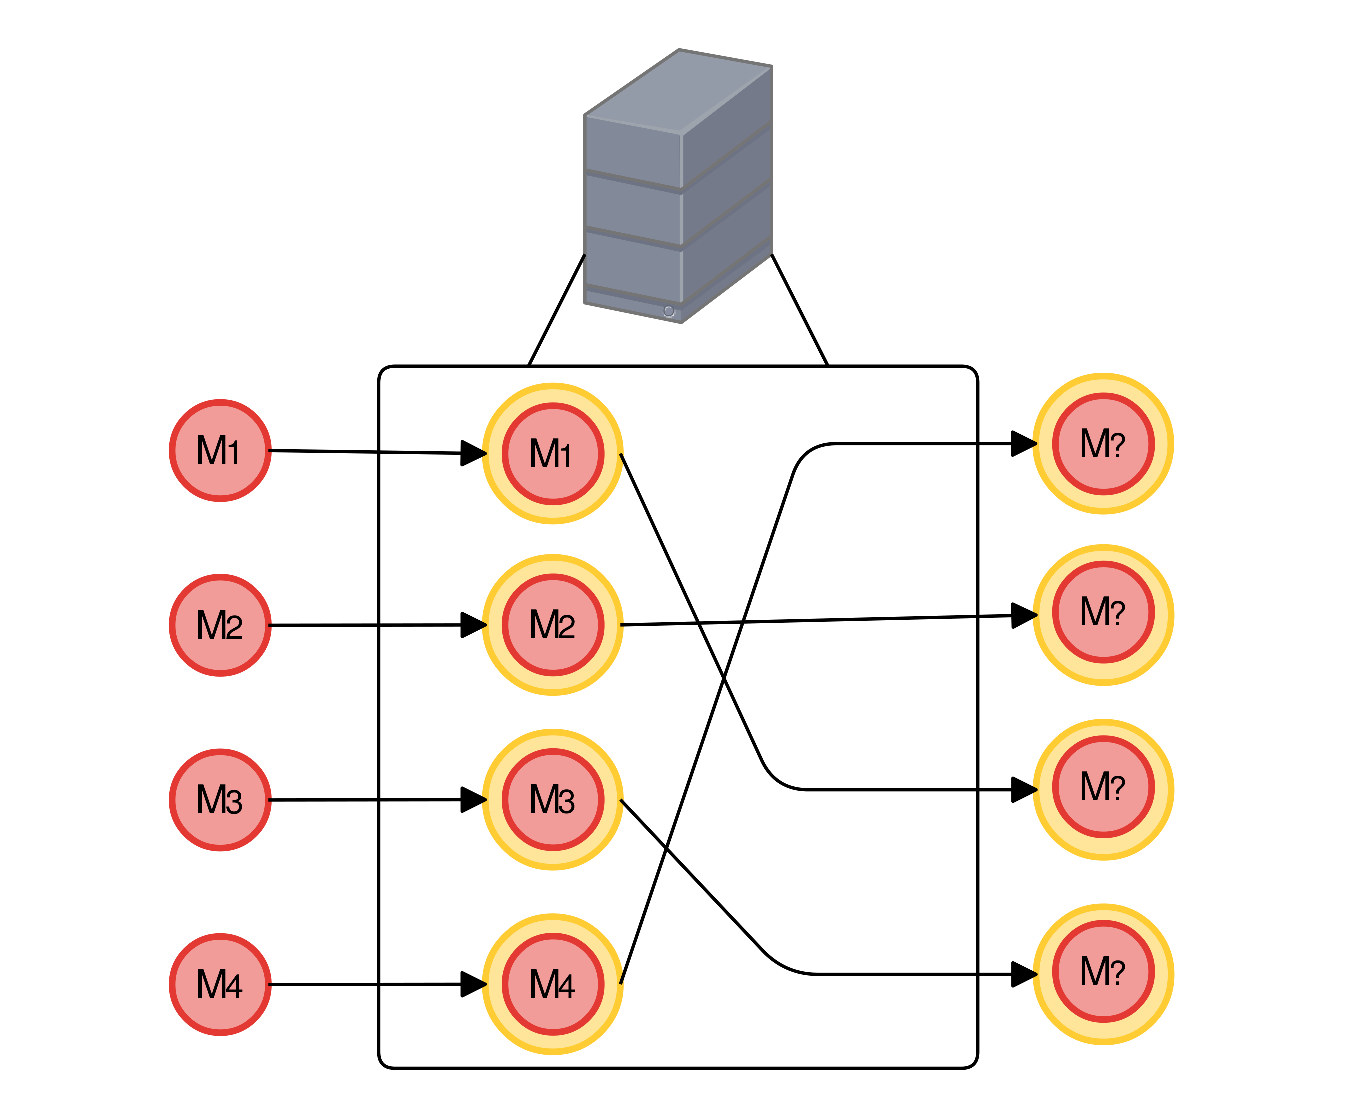
\includegraphics[height=0.7\textheight]{images/mix4.pdf}}
\end{center}

\begin{itemize}
\item El gamal
\end{itemize}

\end{frame}

\begin{frame}{Verifierbarhet}

%Det skapas extra data.

\only<1>{
\begin{center}
  \makebox[\textwidth]{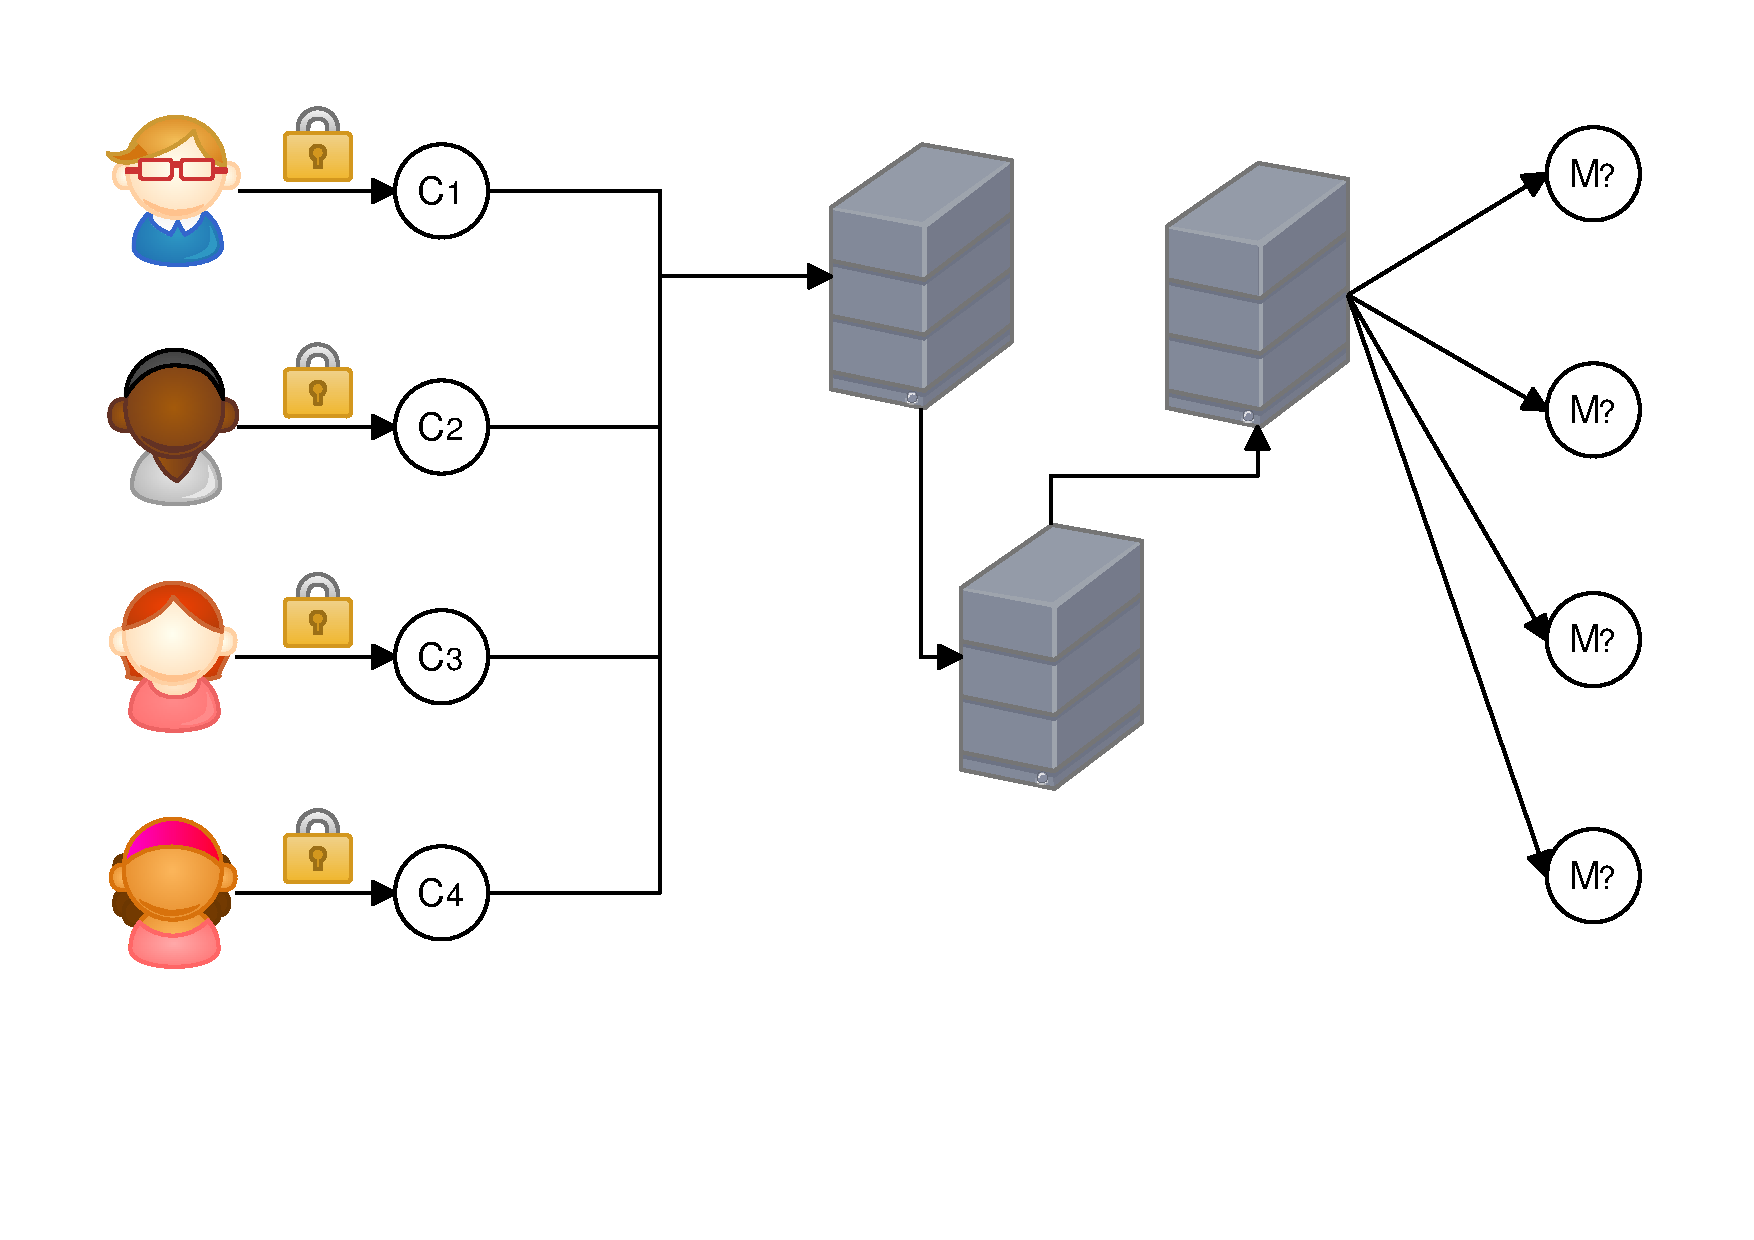
\includegraphics[height=0.6\textheight]{images/mix1.pdf}}
\end{center}
}

\only<2>{
\begin{center}
  \makebox[\textwidth]{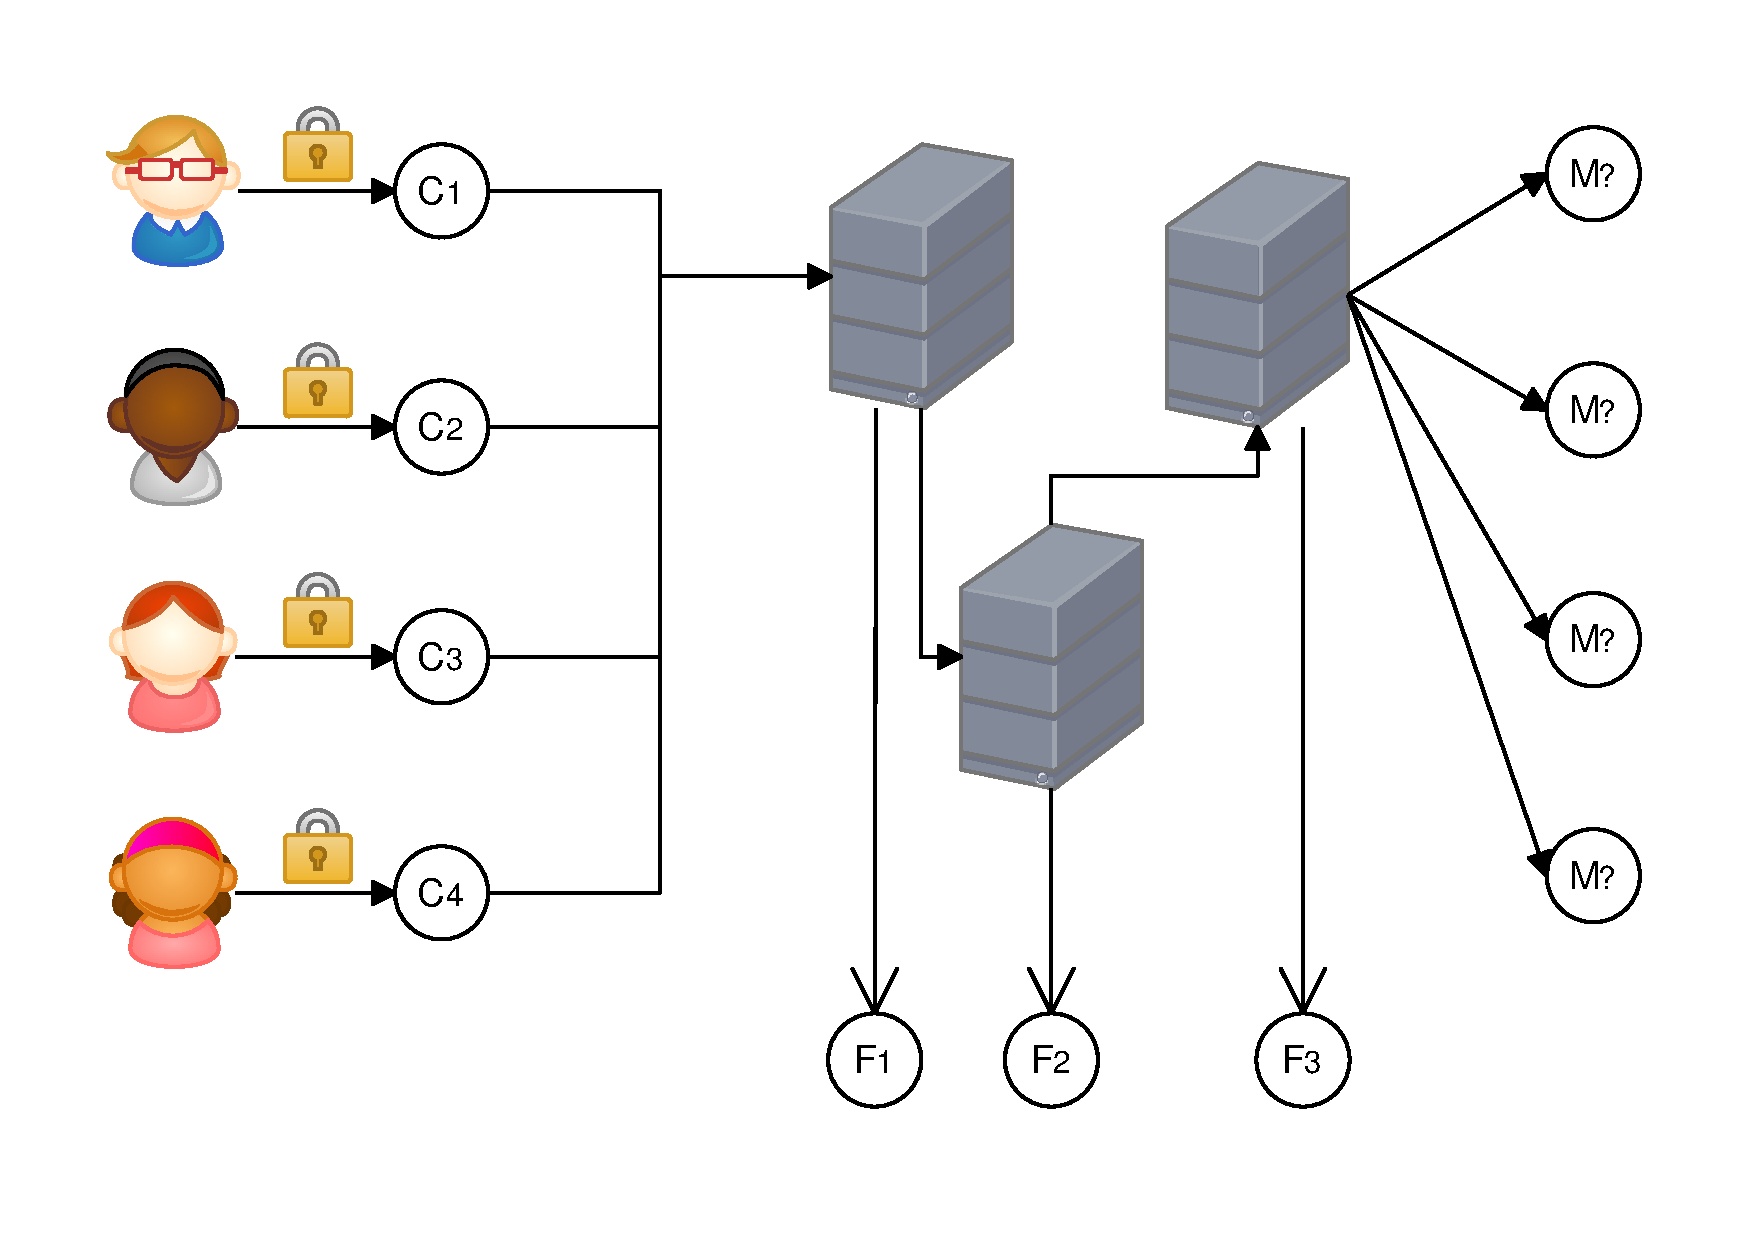
\includegraphics[height=0.6\textheight]{images/mix2.pdf}}
\end{center}
}

\begin{itemize}
\item Verifiering
\item Zero-knowledge
\end{itemize}

\end{frame}

\begin{frame}{Verifiering}

\begin{center}
  \makebox[\textwidth]{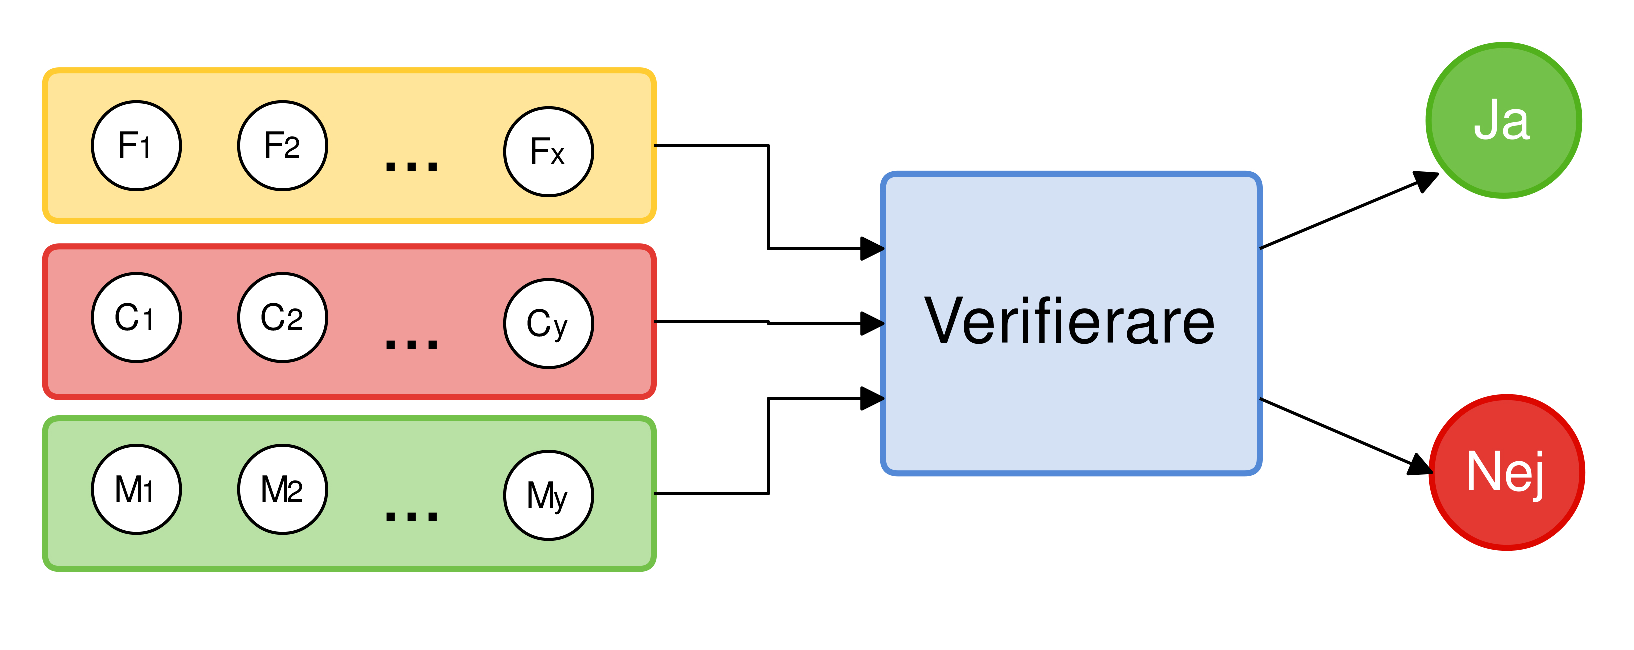
\includegraphics[height=0.9\textheight]{images/mix3.pdf}}
\end{center}

\end{frame}

\begin{frame}{Verifactum}

Implementation, Wikström, titel, CSC

\end{frame}
